
%(BEGIN_QUESTION)
% Copyright 2010, Tony R. Kuphaldt, released under the Creative Commons Attribution License (v 1.0)
% This means you may do almost anything with this work of mine, so long as you give me proper credit

Skisser korrekte slange- og ledningstilkoblinger for å kalibrere denne elektroniske DP-transmitteren til et område på 0 til 40 tommer vannsøyle, med et manometer som trykkstandard og et multimeter for å måle 4-20 mA utgangsstrøm (med positiv strømavlesning). Koble de tre 6-volts batteriene sammen for å lage en 18-volts strømforsyning:

$$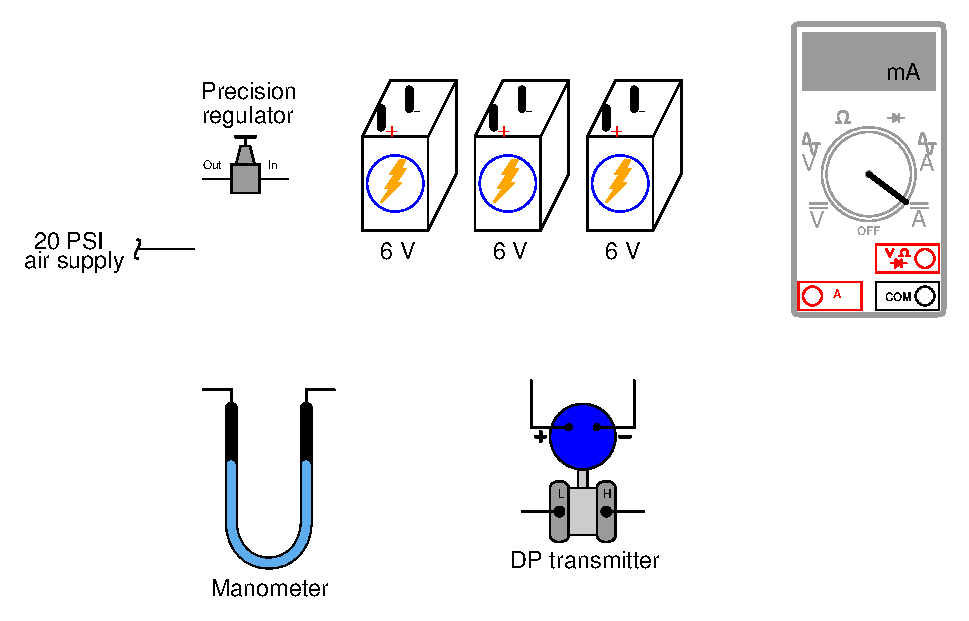
\includegraphics[width=15.5cm]{i01378x01.eps}$$

\underbar{file i01378}
%(END_QUESTION)





%(BEGIN_ANSWER)

Dette er ikke den eneste riktige løsningen. Manometertilkoblingene kan byttes om og likevel fungere helt fint. Amperemeteret kan plasseres enten før eller etter transmitteren i seriekretsen:

$$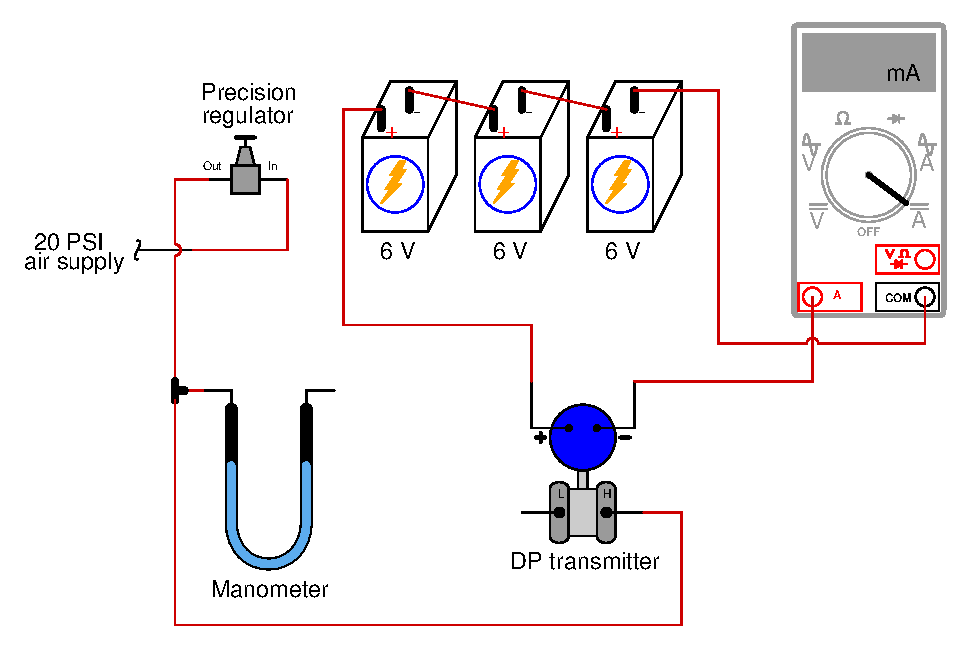
\includegraphics[width=15.5cm]{i01378x02.eps}$$

Trekk 5 poeng dersom multimeteret viser feil polaritet. Ingen poeng dersom kretsen ikke vil fungere slik den er tegnet.

%(END_ANSWER)





%(BEGIN_NOTES)

{\bf Dette spørsmålet er ment kun for eksamener, ikke for arbeidsark!}.

%(END_NOTES)

